% This document is part of the EPRVCalibration project
% Copyright 2019 the authors. All rights reserved.

% style notes
% -----------
% - use \acronym and use \eprv, \lfc, and so on.

\documentclass[12pt, letterpaper]{article}
\usepackage{xcolor}
\newcommand{\lz}[1]{\textcolor{orange}{#1}}

\usepackage[ruled,vlined]{algorithm2e}
\usepackage{graphicx}

% typesetting words
\newcommand{\project}[1]{\textsl{#1}}
\newcommand{\acronym}[1]{{\small{#1}}}
\newcommand{\expres}{\project{\acronym{EXPRES}}}
\newcommand{\name}{\project{NameOfThis}}
\newcommand{\eprv}{\acronym{EPRV}}
\newcommand{\lfc}{\acronym{LFC}}

% math shih
\newcommand{\mps}{\mathrm{m\,s^{-1}}}

% margins and page setup, etc
\addtolength{\textheight}{1.00in}
\addtolength{\topmargin}{-0.50in}
\sloppy\sloppypar\raggedbottom\frenchspacing

\begin{document}

\section*{\raggedright%
\name:
A non-parametric, hierarchical model for a precision spectrograph}

\noindent
\textbf{Lily~Zhao} (Yale) (Flatiron),
\textbf{David~W~Hogg} (NYU) (MPIA) (Flatiron),
\ldots and others\ldots

\paragraph{Abstract:}
There have been many hardware improvements in polygonal-fiber-fed,
temperature-controlled, laser-frequency-comb or etalon-calibrated,
high-resolution, extreme-precision radial-velocity spectrographs.
Have the calibration methodologies improved to match?
Here are three relevant observations:
The first is that the calibration lines or spots from an etalon or
comb (or even arc lamp) fill the spectral range with dense calibration points.
The second is that the spectrograph lives in a stabilized,
climate-controlled environment, in which the full optical system and
detectors will only vary within a tiny range of configurations or
settings.
The third is that, given this stability, every calibration image
ever taken is relevant to every science exposure ever taken; there is
no reason to calibrate every exposure independently.
The calibration methodology we propose here---\name---addresses these
three problems by going non-parametric (no more polynomials!) and then
reducing dimensionality with a robust principal-component method.
We demonstrate the success of this method with data from the
\expres\ spectrograph.
We find... [results and so on].

\section{Introduction} 

Extreme precision radial-velocity (\eprv) programs have been
outrageously successful in finding and characterizing extra-solar
planets (CITE THINGS).
These programs typically make use of spectrographs with resolutions on
the order of $10^5$, which correspond to line widths on the order of
$3000\,\mps$.
Exoplanet science happens at $3\,\mps$ precisions, and the current
instruments hope to get to $0.1\,\mps$ precisions (CITE THINGS).
This means that new spectrographs are expected to be calibrated or
stabilized to better than $10^{-4}$ of a pixel (assuming that the
spectrograph is well sampled).
And indeed, some hardware--software systems seem to be reaching these
levels (CITE THINGS).

Here we propose to simplify and improve calibration programs for
\eprv\ hardware systems with two very simple but novel ideas.
The first flows from the observation that calibration sources---which
include lamps, etalons, and laser-frequency combs (\lfc
s)---illuminate the spectrograph with dense sets of lines; almost every
location in the spectrograph image plane is surrounded by nearby,
useful calibration lines.
This recommends a calibration methodology that is
\emph{non-parametric}:
If every point in the spectrograph detector is surrounded by nearby
calibration lines, the wavelength solution can be made simply an
interpolation of the calibration data.
There is no need to choose any functional form for the wavelength
solution (such as an eighth-order polynomial, for example).
Going non-parametric will improve calibration accuracy, because
choosing a parametric form biases the calibration, and biases it
badly when the form is inappropriate (as, for example, polynomials
will be at the detector edges).

The second idea here flows from the observation that contemporary
\eprv\ instruments are incredibly stable.
Temperature-controlled, fiber-fed pectrographs vary only slightly over
the night or season, and only along a small number of axes in what you
might call ``calibration space'', or the (very high dimensional) space
of all possible wavelength solutions.
That is, not only are they stable, but they don't have many accessible
degrees of freedom.
So it is not appropriate to fit each calibration exposure or calibrate
each science exposure independently.
It makes sense to use the calibration data (or all the data) to
determine the space in which the instrument can and does vary, and
then in subsequent calibration work only permit the solution to live
in the accessible part of calibration space.
This structure is \emph{hierarchical}: The calibration data are used
not just to determine the wavlength solution, but also to determine
the possible space of wavelength solutions.
In the statistics literature this concept is often described as
\emph{de-noising}:
Every calibration exposure contains information about every other
exposure; it doesn't just constrain the instrument locally in time.
Thus every exposure can be improved (de-noised) with information
coming from every other exposure.

The method we propose here---\name---embodies these ideas.
It is a non-parametric, hierarchical, data-driven model for the
wavelength solution.
By being non-parametric, it delivers enormous freedom to the
wavelength solution to match or adapt to any instrument or detector
oddities.
By being hierarchical, it restricts that freedom tremendously, but it
does so appropriately for the observed variations in the
spectrograph.
\name\ is designed for temperature-controlled, bench-mounted, fiber-fed
spectrographs with good calibration sources, such as laser-frequency
combs, etalons, or good arc lamps.
We have in mind the \eprv\ instruments and \eprv\ science cases.
But we expect \name\ to have applications for other kinds of
spectrographs in other contexts; the motivating ideas behind this
project are true for almost every astronomical spectrograph.

\section{Method} \label{sec:method}
We operate on the two core ideas that the wavelength solution should be given enormous flexibility, but that in fact it will be living in a very low-dimensional space, where the degrees of freedom are set by the limited kinematics of the spectrograph hardware.

HOGG: THIS IS NOW ALL WRONG... We will pose the problem in the following way.  Given an exposure $n$, and order $m$, there is a relationship between
the two-dimensional $(x,y)$-position on the detector and the
wavelength $\lambda$
\begin{equation}
\lambda(x,y,m,n) = f(x,y,m;\theta_{n})
\quad ,
\end{equation}
where $\theta_{n}$ is a big blob of parameters for this exposure.

A stabilized spectrograph should experience only low-degree variability, meaning the calibration of any image can be informed by the calibration of every other image.  To implement such a hierarchical model, we use the calibration data themselves to develop a low-dimensional basis for expressing the calibration data.

If the space of all calibration possibilities is in fact $K$-dimensional (where K is a small integer, i.e 2 or 8 or thereabouts), and if the calibration variations are so
small that we can linearize, then the function $f(x,y,m;\theta_{n})$ could
be replaced with a tiny model
\begin{equation}
\lambda(x,y,m,n) = g_0(x,y,m) + \sum_{k=1}^K a_{nk}\,g_k(x,y,m)
\quad ,
\end{equation}
where
$g_0(x,y,m)$ is the fiducial or mean or standard calibration of the
spectrograph,
the $a_{nk}$ are scalar amplitudes,
and the $g_k(x,y,m)$ are basis functions expressing the ``directions'' in calibration space that the spectrograph can depart from the
fiducial calibration.
The challenge is to learn these basis functions from the data and get
the $K$ amplitudes $a_{nk}$ for every exposure $n$.

\subsection{Data} \label{sec:data}
We present results using data from \expres\, the EXtreme PRecison Spectrograph.  \expres\ is an envionmentally stabilized, fiber-fed, $R=137,000$, optical spectrograph (\lz{CJ and RB's papers}).  \expres\ has two different wavelength calibration sources, a ThAr lamp and a Menlo Systems laser frequency comb (LFC, e.g. \lz{Wilken+ 2012, Molaro+ 2013, Probst+ 2014, from RB's paper}).  ThAr exposures are taken at the beginning and end of each night.  LFC exposures are interspersed between science exposures every ~15 minutes.  
(Discussion of number of orders covered or number of lines in LFC and/or ThAr?)

\lz{Discussion of line fitting?  Though the current line fitting causes me recurring nightmares.  I should really take the time to look into at least the peak fitting more.}

For the results presented in this paper, we work with the 1D, optimally extracted data.  This removes the y-dependence from equations 1 and 2.

\expres\ exposures are separated into different ``instrumental epochs," which correspond to changes to the position of the echellogram on the detector, the shape of the instrumental PSF, or the calibration sources (\lz{(worth including table that explicitly defines epochs?)}).  Because significant instrumental changes break the assumption of only low-dimensional variations in the spectrograph hardware, we treat each instrument epoch independently.

\subsection{Hierarchical De-Noising of Calibration Frames} \label{sec:denoising}
Let $\{exp_n\}$ be the set of calibration exposures within an instrument epoch used to construct $g_k(x,y,m)$.  We first identify the full list of lines we can expect to find in a calibration image from this epoch.  A line is uniquely defined by a combination of order, $m$, and ``true" or theoretical wavelength of that line, $\lambda$.  Let $\{l_{m,\lambda}\}$ be the complete list of unique lines found in $\{exp_n\}$.

For each line, $l_{m,\lambda}$, we then find the fitted line center, $x_{n,l}$, in pixel space, for that line for each exposure.  If this line is missing from an exposure (e.g. it was covered by noise or off the edge of its usual order), we insert a $NaN$ for that line center instead.

Lines that are missing from greater than some percent of exposures are cut.  Exposures that are missing greater than some percent of lines are also cut (\lz{This will miss low signal exposures that suffer most in the first few orders but can recover in later orders; can't decide if this is a feature or a bug}).  This threshold percentage is 50\% for LFC exposures and 30\% for ThAr exposures.

Missing line center measurements are replaced with denoised estimates using iterative PCA.  For each missing line center measurement, we initialzie their value to the mean of the nearest $n$ exposures in time, where $n$ is typically 9 for LFC exposures and $15$ for ThAr.  We then find a fiducial calibration of the spectrograph,  $g_0(x,y,m)$, for which we use the mean line center value for each identified line.  We subtract this fiducial calibration from each exposure's measured line centers and run PCA on the difference between the measured and fiducial line center for each exposure.  This PCA gives us $a_{nk}$ and $g_k(x,y,m)$.

Using those values with equation 2 and some small integer (e.g. 2) for K, we can reconstruct a de-noised matrix of line centers for each exposure.  Missing line center measurements are then replaced with values from this reconstruction.  We do this iteratively until the values of the missing line centers change by less than 0.01\% of a pixel.  This convergence suggests that the PCA is no longer being swayed by outliers and is truly ``de-noised."

\begin{algorithm}
\SetAlgoLined
\textbf{Inputs}: \;
\While{change in bad pixels $>$ 0.01\%}{
	$g_0(x,y,m) = \overline{\{x_{n,l}\}}$\;
	find $U, \Sigma, V$ s.t. $U\Sigma V^* = (x_{l,n}-g_0(x,y,m))$\;
	let $a_{n,k} = U\cdot \Sigma$ and $V = g_k(x,y,m)$\;
	$\lambda(x,y,m,n) = g_0(x,y,m) + \sum_{k=1}^K a_{nk}\,g_k(x,y,m)$ where $K=2$\;
	$\{x_{n,l}\} = \lambda(x,y,m,n)$ where $\{x_{n,l}\}$ is $NaN$
	}
\caption{Hierarchical De-Noising}
\end{algorithm}

\subsection{Non-Parametric Calibration} \label{sec:nonparam}
We can interpolate $a_{nk}$ with respect to time to determine $\lambda(x,y,m,n)$ at any time.  Once we have the line center for each line, which has an associated known wavelength, we can interpolate the known wavelengths over line centers to any position in x in a given order.  For example, interpolating onto every integer x will generate wavelengths for each pixel in an order.

We chose to implement both interpolations with a cubic spline.  Interpolation of wavelengths over line centers is done order by order.

\begin{algorithm}
\SetAlgoLined
\textbf{Inputs}: new time, new line centers, new orders\; %command not working for w/e reason
Let $t_n$ be the time associated with exposure $n$\;
let $t_n'$, $x_n'$, and $m_n'$ be the new time, line centers, and orders we want wavelengths for\;
Let $a_{n,k}'$ be the interpolation of $a_{n,k}$ to time $t_n'$\;
$\lambda(x,y,m,n)' = g_0(x,y,m) + \sum_{k=1}^K a_{nk}'\,g_k(x,y,m)$ where $K=2$\;
\For{each unique $m_n'$}{
	${l_n,m}$ from $\lambda(x,y,m,n)'$
	interpolate ${l_n,m}$ onto $x_n'$\;
	}
\caption{Non-Parametric Wavelength Solution}
\end{algorithm}
\lz{What's fancy math symbol for interpolate?}

\subsection{Choice Choices} \label{sec:choices}
(Before or after results presented in validation test and ThAr sections?)

We're still testing most of these (will use that as excuse to write this section later)
\begin{itemize}
	\item Value of K for denoising
	\item Type of interpolation (cubic spline vs nearest neighbor or linear)
	\item Interpolation order (interpolate time and x direction together?  Individually?  Which one first?)
\end{itemize}

Reason for not linear interpolation:
Due to the dispersion intrinsic to echelle spectrographs, the wavelength change between pixels is greater at greater wavelengths.  This means that the function of wavelength given pixel across an order will necessarily be concave down everywhere.  Consequently, linear interpolation of this function will systematically give erroneously low values.


\section{Results} \label{sec:results}
\subsection{Self Tests} \label{sec:test-self}
First, let's have a sanity check.  Using a cubic spline scheme with no smoothing to predict wavelengths for the returned, denoised line center values, $\lambda(x,y,m,n)$, should return identical values to the assigned true wavelength for each line within machine error.
This is what happens, for both ThArs and LFCs: look at the figure.

As an only slightly less silly sanity check, we can also use the constructed PCA basis to predict wavelengths for the measured line centers of an exposure that was included in the set of exposures used to construct the basis.  This interpolation should return identical PCA coefficients for that time.  Differences in wavelengths will arise from a combination of 1) the error inherent in measuring line centers and 2) interpolation error of lines to other x positions in the pixel direction.

Difference in denoised x-values to measured ones? (translate into rv shift?)
median and spread in errors in pixel (like 0.006) and RV (like 3.2 m/s?)
Histograms

\subsection{Training and Validation Tests} \label{sec:test-trainNvalid}
A better test is to leave out some percentage of the calibration images from $\{exp_n\}$ while constructing the basis and weights with PCA.  We can then use the results from that PCA to predict wavelengths for lines in the calibrations images that were left out.  We will call the used calibration images the ``training set," and the left out exposures the ``validation set."

We chose to use 90\% of available exposures to train the PCA, and leave the remaining 10\% for validation.  Exposures were sorted into either set at random.  This will test how well PCA coefficients are interpolated to other times outside of the training set and therefore how well line centers can be reconstructed at all times.  As before, differences in wavelength will also be drawn from how well line centers are measured and error in interpolating to those measured values.  This second source of error was independently quantified in the second test described in the previous section.

LFC looks good, ThAr is struggling a bit
Difference in denoised x-values to measured ones? (translate into rv shift?)
median and spread in errors in pixel (like 0.006) and RV (like 3.2 m/s?)
Histograms

\subsection{Cross Tests} \label{sec:test-cross}
Similar to the training and validation tests, we can also use one calibration source to construct the PCA basis and weights and the other to test the results.  For example, we can use LFC exposures to construct the wavelength solution, and then use it to predict wavelengths for measured line centers of ThAr lines, which will have their own assigned true wavelengths.  Likewise, we can use ThAr exposures to predict the wavelengths of LFC lines.  Note that errors in this test will also draw on the difference in quality of the two calibration sources being compared.

LFC predicts ThAr better than ThAr can predict itself.
ThAr predicting LFC is really messing up somehow, and I should figure out what it is (sorry!)

%\subsection{ThAr Stuff?  Or Include it in Previous Subsections?}

\section{Comparisons to Other Methods} \label{sec:comparisons}
I think we probably have to use the even/odd method to compare.

\subsection{Comparison to Parametric Model}
Previously, the \expres\ pipeline the $\theta_{n}$ from equation 1 comprises the
amplitudes of some 9th-ish-order polynomial in $x$ and $m$ for each $n$.
If so, they have
\begin{equation}
\lambda(x,y,m,n) = \sum_{i=0}^9\sum_{j=0}^9 c_{nij}\, x^i\,m^j + \mathrm{noise}
\quad ,
\end{equation}
where the $c_{nij}$ are coefficients unique to exposure $n$ but smoothed by a third order polynomial over time.
Further, they were finding the coefficients $c_{nij}$ that
minimize an objective $Q$ that is something like the L2-norm:
\begin{equation}
Q = ||\lambda(x,y,m,n) - \sum_{i=0}^9\sum_{j=0}^9 c_{nij}\, x^i\,m^j||_2^2
\quad .
\end{equation}

Even in this simple context, where every calibration image $n$ is
treated as its own unique flower, there are improvements to be
made.
For one, the sums should not be from 0 to 9, but instead
\begin{equation}
\sum_{i=0}^9\sum_{j=0}^{9-i}
\quad ,
\end{equation}
because that is the definition of 9th order.  We find that fitting to 8th order is sufficient, faster, and leaves less residual pattern than the original 9th degree fit.
For another, the objective function could be made soft to permit
catastrophic outliers without destroying the fit. (\lz{we did not do this})
We might recommend the iteratively reweighted least squares (IRLS).
This would make the fitting more robust.
For yet another, there are rescaling issues for the products $x^i\,m^j$ to
protect the fitting from near-singularities or bad conditioning of the
linear-algebra operators.


\begin{figure}[h]
\centering
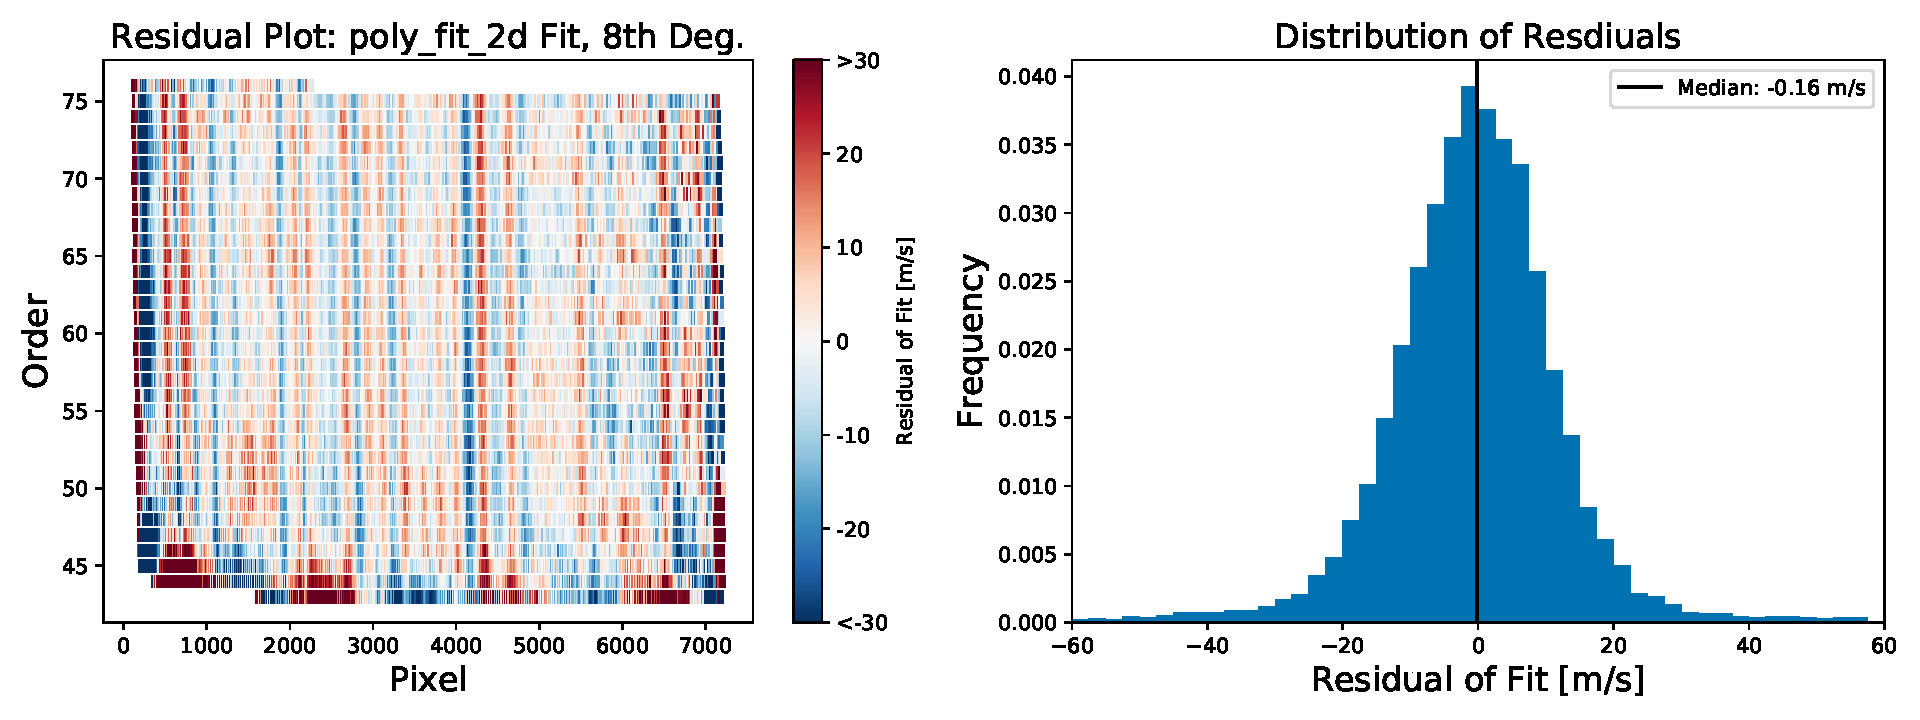
\includegraphics[width=0.9\textwidth]{Figures/polyval2d.pdf}
\caption{}
\label{fig:polyValFit}
\end{figure} 

\begin{figure}[h]
\centering
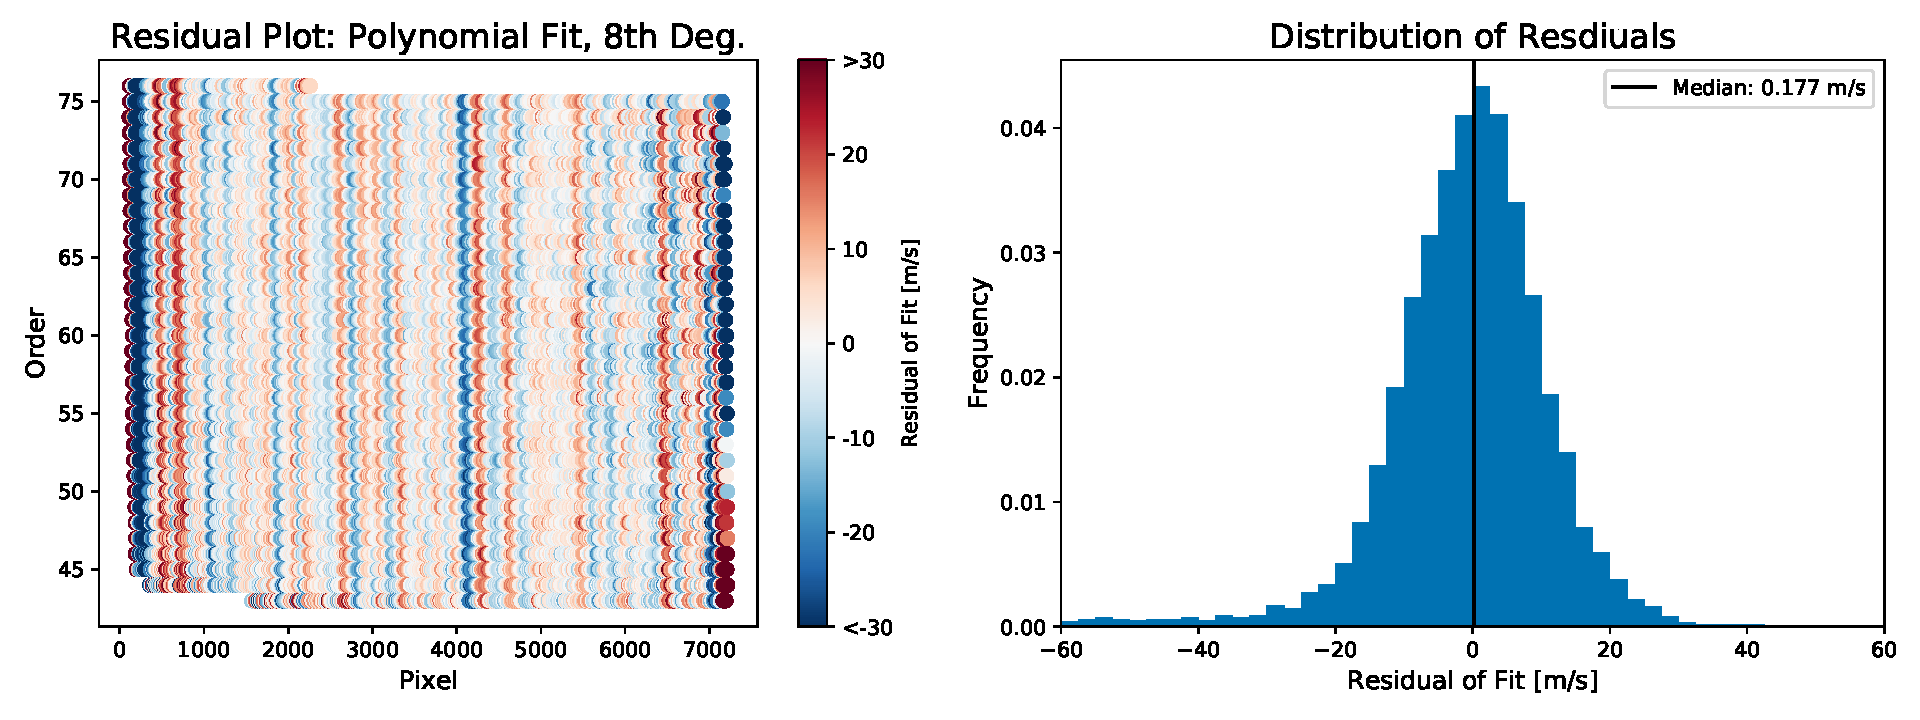
\includegraphics[width=0.9\textwidth]{Figures/designMatrix.pdf}
\caption{}
\label{fig:dsnMFit}
\end{figure} 

\subsection{Comparison to Non-Parametric, Non-Hierarchical Model}

\begin{figure}[h]
\centering
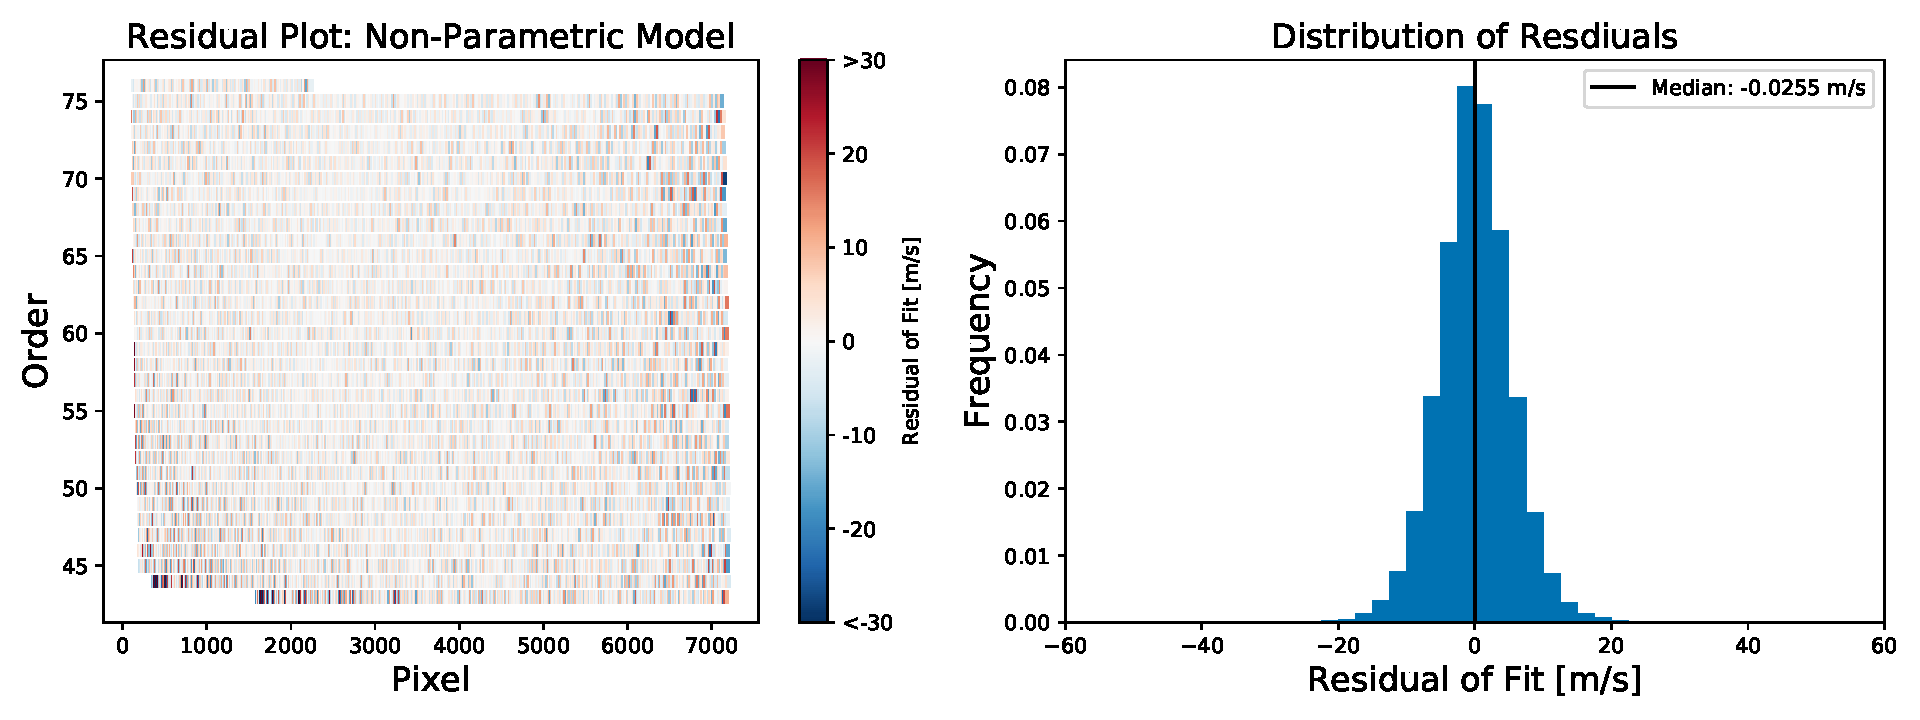
\includegraphics[width=0.9\textwidth]{Figures/noHierc.pdf}
\caption{}
\label{fig:intpFit}
\end{figure} 

\section{Real Data Through to RVs} \label{sec:realdata}

\section{Discussion} \label{sec:discussion}

Generalization to etalon

Maybe some practical statements?  How many exposures are needed to implement this method at all.  How often do exposures have to be taken throughout a night (unless that's too dependent on instrument stability)

Some ideas about self-calibration. Once you know the space in which the
spectrograph lives, every single science frame gives you information about
where you are in that space; you don't need to look at the \lfc.

\end{document}
